\documentclass[a4paper,12pt]{article}
\usepackage{amsmath,amssymb}
%\usepackage[utf8]{inputenc}
%\usepackage[applemac]{inputenc}
\usepackage{geometry}
\usepackage{lscape}
\usepackage{setspace}
\usepackage{framed}
\usepackage{verbatim}
\usepackage{graphicx}
\usepackage{epstopdf}
\usepackage{booktabs}
\usepackage{natbib}
%\usepackage{longtable}
%\usepackage{rotating}                                                                                    
\newcommand{\tab}{\hspace{5mm}}
\usepackage{tabularx} 
\usepackage[margin=10pt,font=small,labelfont=bf]{caption}
\usepackage[left,pagewise]{lineno}
%\usepackage{caption}
\DeclareGraphicsRule{.tif}{png}{.png}{`convert #1 `basename #1 .tif`.png}
\usepackage{fancyhdr} % This should be set AFTER setting up the page geometry
\pagestyle{fancy}     % options: empty , plain , fancy
\renewcommand{\headrulewidth}{0pt} % customise the layout...
\lhead{{\tiny Jordano - Sampling networks}}\chead{}\rhead{}
\lfoot{}\cfoot{\thepage}\rfoot{}
\setlength{\parskip}{\baselineskip} % increase paragraph separation
%
\def\mytitle{Sampling interactions manuscript}
\def\myauthor{Pedro Jordano}
\def\mydate{February 24, 2015}
\def\comment{Manuscript draft for the sampling interactions study.}
\def\bibliocommand{\bibliography{refs}}
\def\bibliographystyle{pnas}
%
%%%%%%%%%%%%%%%%%%%%%%%%%%%%%%%%%%%%%%%%%%%%%%%%%%%%%%%%%%%%%%%%%% Title page
\begin{document}
\title{Manuscript Draft\\
\vspace{2cm}
Sampling ecological interaction networks}

\author{Pedro Jordano$^{\dag}$}

\date{Sevilla, \today}
\maketitle


\begin{spacing}{1.0}
$^{\dag}$ {\small Integrative Ecology Group, Estaci\'on Biol\'ogica de 
Do\~nana, CSIC, Pabell\'on del Per\'u, Avda. Mar\'ia Luisa, s/n, 
E-41013 Sevilla, Spain.}\\


{\small \textit{Corresponding author:} Pedro Jordano. Integrative Ecology Group, Estaci\'on Biol\'ogica de Do\~nana, CSIC, Pabell\'on del Per\'u, Avda. Mar\'ia Luisa, s/n, E-41013 Sevilla, Spain. Fax number: +34 95 4621125. Email address: jordano@ebd.csic.es}\\

\textbf{Key words}: ***\\

{\small \textbf{Manuscript information: }** Words; ** Chars; ** Pages, * Figures; * Tables.}
\maketitle
\newpage
%%%%%%%%%%%%%%%%%%%%%%%%%%%%%%%%%%%%%%%%%%%%%%%%%%%%%%%%%%%%%%%%%%%%%%%%%%%%%%%%
\begin{center}\rule{3in}{0.4pt}\end{center}


\chapter{Abstract}
\label{abstract}

Sampling ecological interactions presents similar challenges, problems, potential biases, and constraints as sampling individuals and species in biodiversity inventories. Interactions are just pairwise relationships among individuals of two unrelated species, such as those among plants and their seed dispersers in frugivory interactions or those among plants and their pollinators. Sampling interactions is a fundamental step to build robustly estimated interaction networks, yet few analyses have attempted a formal approach to their sampling protocols.
Here I provide a review and conceptual framework for interaction sampling by building an explicit analogue to individuals and species sampling, thus extending diversity-monitoring approaches to the characterization of complex networks of ecological interactions. 

\begin{center}\rule{3in}{0.4pt}\end{center}


\chapter{Introduction}
\label{introduction}

\begin{verbatim}
Biodiversity sampling is a labour-intensive activity,   
and sampling is often not sufficient to detect all or   
even most of the species present in an assemblage.   

Gotelli & Colwell (2011).
\end{verbatim}

Biodiversity assessment aims at sampling individuals in collections and determining the number of species represented. Given that, by definition, samples are incomplete, these collections enumerate a lower number of the species actually present. The ecological literature dealing with robust estimators of species richness and diversity in collections of individuals is immense, and a number of useful approaches have been used to obtain such estimates \citep{Magurran:1988mm}\citep{Gotelli:2001uo}\citep{Hortal:2006dc}\citep{Gotelli:2011tb}. Recent effort has been also focused at defining essential biodiversity variables (EBV) [Pereira:2013ji] that can be sampled and measured repeatedly to complement biodiversity estimates. Yet sampling species or taxa-specific EBVs is just probing a single component of biodiversity; interactions among species are another fundamental component, the one that supports the existence of species \citep{Memmott:2006vy}. For example, the extinction of interactions represents a dramatic loss of biodiversity because it entails the loss of fundamental ecological functions \citep{ValienteBanuet:2014bw}. This missed component of biodiversity loss, the extinction of ecological interactions, very often accompanies, or even precedes, species disappearance. I can't emphasize enough the relevance of sampling interactions in addition to sampling species and higher taxa in biodiversity assessment programs. Interactions among species are a key component of biodiversity and here I aim to show that most problems associated to sampling interactions in natural communities have to do with problems associated to sampling species diversity. In the first part of this paper I provide a succinct overview of previous work addressing sampling issues for ecological interaction networks. In the second part I discuss specific rationales for sampling the biodiversity of ecological interactions.
 Interactions in natural ecosystems can be a much better indicator of the richness and diversity of ecosystem functions than a simple list of taxa and their abundances and\slash or related biodiversity indicator variables (EBVs). Thus, sampling interactions should be a central issue when identifying and diagnosing ecosystem services (e.g., pollination, natural seeding by frugivores, etc.). Fortunately, all the whole battery of biodiversity-related tools used by ecologists to sample biodiversity (species, \emph{sensu stricto}) can be extended and applied to the sampling of interactions. Analogs are evident between these approaches. Monitoring interactions is analogous to any biodiversity sampling (i.e., a species inventory \citep{E31/2562}\citep{Jordano:2009c}) and is subject to similar methodological shortcomings, especially under-sampling \citep{Coddington:2009fi}\citep{Vazquez:2009p82}\citep{Dorado:2011cf}. When we study mutualistic networks, our goal is to make an inventory of the distinct pairwise interactions that made up the network. We are interested in having a complete list of all the pairwise interactions among species (e.g., all the distinct, species-species interactions, links, among the pollinators and flowering plants) that can exist in a given community. And sampling interactions entails exactly the same problems, limitations, constraints, and potential biases as sampling individual organisms and species diversity. 

[Review part]
 Earlier efforts to recognize and solve sampling problems in analyses of interactions stem from researchers interested in food web analyses and in determining the biases on undersampled food web metrics \citep{Bersier:2002p9371}\citep{Brose:2003wv}\citep{BanasekRichter:2004ik}. In addition, the myriad of natural history studies documenting animal diets, host-pathogen infection records, plant herbivory records, etc., are basic efforts to document interactions occurring in nature. All of them share the problem of sampling incompleteness influencing the patterns and metrics reported. Yet, despite the recognition that incomplete sampling may seriously bias the analysis of ecological networks \citep{E31/2562}, only recent studies have explicitly acknowledged it and attempted to determine its influence \citep{Ollerton:2002jw}\citep{Nielsen:2007}\citep{Vazquez:2009p82}\citep{Gibson:2011eh}\citep{Olesen:2011a}\citep{Chacoff:2012}\citep{RiveraHutinel:2012vn}[Fründ, McCann \& Williams 2015]. Most studies provide no estimate of sampling effort, implicitly assuming that the reported network patterns and metrics are robust (i.e., additional sampling would not entail significant modifications of the reported results).
 To date, only a handful of studies have explicitly evaluated the effects of sampling incompleteness on the description of network structure. These studies found high variation in the number of detected species and total number of links and suggest that some metrics, i.e. aggregated statistics describing network patterns, are prone to sampling bias (e.g. Goldwasser \& Roughgarden 1997, Martinez et al. 1999, Banašek-Richter, Cattin \& Bersier 2004, Nielsen \& Bascompte 2007, Rivera-Hutinel et al. 2012, Fründ, McCann \& Williams 2015). Nevertheless, some important gaps remain to be addressed regarding the importance of sampling completeness. Notably, little is known about the influence of sampling effort on quantitative network structure, i.e. metrics calculated from networks that take into account the strength of interactions, and there has been no attempt at investigating the effects of sampling incompleteness on the understanding of the processes structuring ecological networks. Furthermore, practically all information about the influence of sampling on detected network structures are based on either simulated networks (e.g. Fründ, McCann \& Williams 2015) or are from species-poor ecosystems, such as desert or temperate forests (e.g. Nielsen \& Bascompte 2007; Chacoff et al. 2012, Rivera-Hutinel et al. 2012), whereas incomplete sampling should be greatest in networks from species-rich tropical regions (Ollerton \& Cranmer 2002; Kissling \& Schleuning 2015).

\chapter{Sampling interactions: methods}
\label{samplinginteractions:methods}

When we sample interactions in the field we record the presence of two species that interact in some way, i.e., a frugivorous pigeon visits a fruiting tree and detaches and ingests the fruit of a given plant species. For example, Snow and Snow\citep{Snow:1988iu} recorded an interaction whenever they saw a bird ``touching'' a fruit on a plant. In a similar way, interactions between pollinators and plants are tallied by recording any visit of a pollinator entering a flower and touching the androceum and\slash or the gyneceum. We observe and record feeding observations, visitation, occupancy, presence in pollen loads or in fecal samples, etc., of individuals animals or plants to accumulate pairwise interactions, i.e., lists of species partners and the frequencies with which we observe them. Therefore, estimating the sampling completeness of plant–animal interactions for the whole network, requires estimating the number (richness) of distinct pairwise interactions accumulated as sampling effort is increased, pooling the data for all plant and animal species.
 Sampling interactions requires filling the cells of an interaction matrix with data. The matrix, $AP$, is a 2D representation of the interactions among $A$ animal species (rows) and $P$ plant species (columns) \citep{E31/2562}\citep{Bascompte:2014to}. An interaction matrix $AP$ consists of an array of zeroes or ones, or an array of zeroes and numbers- if the data (interaction frequencies) are quantified. These figures illustrate the values of the pairwise interactions visualized in the $AP$ matrix.
 We need to define two basic steps in the sampling of interactions: 1) which type of interactions we sample; and 2) which type of record we get to document the existence of an interaction. In step \#1 there are two considerations we need to take into account. First is whether we are sampling the whole community of interactor species (all the animals, all the plants) or we sample a subset of them. Subsets can be: a) We sample all the potential plants interacting with a subset of the animals; b) We sample all the potential animal species interacting with a subset of the plant species; c) We sample a subset of all the potential animal species interacting with a subset of all the plant species.

\subsubsection{Fig. 1 here}
\label{fig.1here}

\begin{figure}[htbp]
\centering
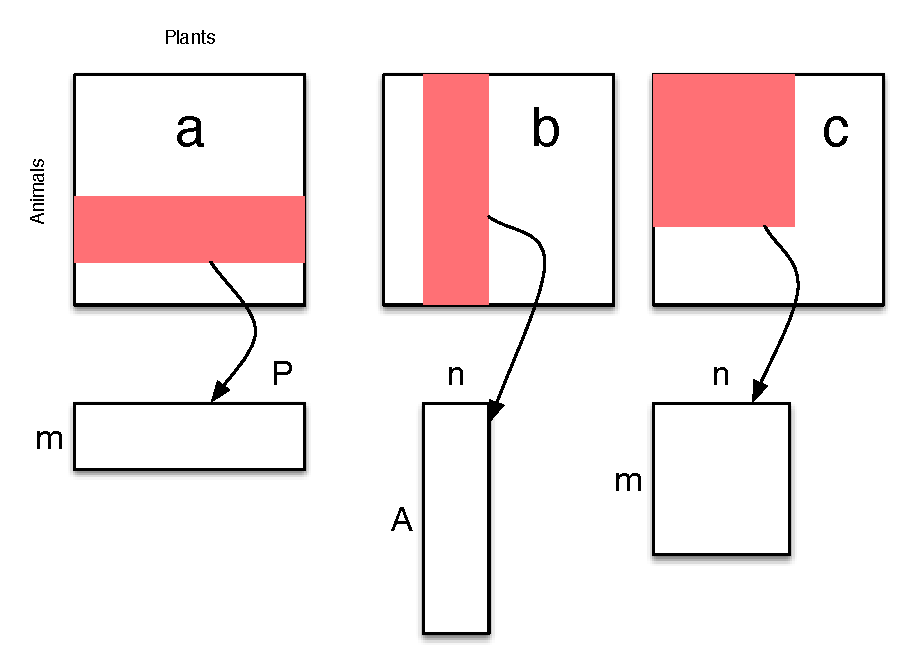
\includegraphics[keepaspectratio,width=\textwidth,height=0.75\textheight]{../figures/Fig1.pdf}
\caption{Figure 1. Sampling ecological interaction networks usually focus on different types of subsampling the full network. a) all the potential plants interacting with a subset of the animals (e.g., studying just the hummingbird-pollinated flower species in a community); b) all the potential animal species interacting with a subset of the plant species (e.g., studying the frugivore species feeding on figs \emph{Ficus} in a community); and c) sampling a subset of all the potential animal species interacting with a subset of all the plant species (e.g., studying the plant-frugivore interactions in the rainforest understory).}
\end{figure}

In step \#2 above we face the problem of the type of record we take to sample interactions. This is important because it defines whether we approach the problem of filling up the interaction matrix in a ``zoo-centric'' way or in a ``phyto-centric'' way. We could use a conceptual table to illustrate a summary of these two types of approaches for the analysis of frugivory, pollination, and herbivory interactions; just summarize, $A$, $P$, $I$ and $C$ for a number of case studies grouped according to whether they are zoo-centric or phyto-centric. Zoo-centric studies directly sample animal activity and document the plants `touched' by the animal. E.g., analysis of pollen samples recovered from the body of pollinators, analysis of fecal samples of frugivores, radio-tracking data, etc.
Phyto-centric studies take samples of focal individual plant species and document which animals `arrive' or `touch' the plants. Examples include focal watches of fruiting or flowering plants to record visitation by animals, raising insect herbivores from seed samples, identifying herbivory marks in samples of leaves, etc.

\begin{verbatim}
We can discuss whether zoo-centric or phytocentric sampling potentially bias the estimation of interactions.
\end{verbatim}

\chapter{Sampling interactions: rationale}
\label{samplinginteractions:rationale}

Independently of whether we sample full communities of subset communities we face a problem: some of the interactions that we can visualize in the empty matrix $AP$ will simply not occur. Thus, independently of the sampling effort we put, we'll never document these pairwise interactions. With a total of $AP$ interactions possible, a fraction of them are impossible to record, because they are forbidden \citep{E31.7324_PDF}\citep{Olesen:2011a}. Forbidden links are constraints for the establishment of new links, and mainly arise from the biological attributes of the species: no link can be established between a plant and an animal mutualist differing in phenology, i.e. the seeds of a winter-ripening plant cannot be dispersed by a frugivore that is a summer stopover migrant \citep{E31/2562}. Or, for instance, short-tongued pollinators cannot successfully reach the nectar in long-corolla flowers and pollinate them efficiently \citep{More:2012kx}. Forbidden links are thus represented as structural zeroes in the interaction matrix, i.e., matrix cells that cannot get a non-zero value. So, we need to account for the frequency of these structural zeros in our matrix before proceeding. For example, most measurements of connectance ($C= I/(AP)$) implicitly ignore the fact that by taking the full product $AP$ in the denominator they are underestimating the actual connectance value.
 The number of distinct pairwise interactions that we can record in a landscape (an area of relatively homogeneous vegetation, analogous to the one we would use to monitor species diversity) is equivalent to the number of distinct classes in which we can classify the recorded encounters among individuals of two different species. We walk in the forest and see a blackbird $Tm$ picking an ivy $Hh$ fruit and ingesting it: we have a record for $Tm-Hh$ interaction. We keep advancing and record again a blackbird feeding on hawthorn $Cm$ fruits so we record a $Tm-Cm$ interaction; as we advance we encounter another ivy plant and record a blackcap swallowing a fruit so we now have a new $Sa-Hh$ interaction, and so on. At the end we have a series of classes (e.g., $Sa-Hh$, $Tm-Hh$, $Tm-Cm$, etc.), along with their observed frequencies. Bunge \& Fitzpatrick \citep{Bunge:1993ux} review the main aspects and approaches to estimate the number of distinct classes $C$ in a sample of observations. The sampling of interactions in nature, as the sampling of species, is a cumulative process. We add new, distinct, interactions recorded as we increase sampling effort (Fig. 1). We can obtain an Interaction Accumulation Curve ($IAC$) analogous to a Species cumulating Curve ($SAC$): the observed number of distinct pairwise interactions in a survey or collection as a function of the accumulated number of observations or samples\citep{Colwell:2009gv}. 

\subsubsection{Fig. 2 here}
\label{fig.2here}

\begin{figure}[htbp]
\centering
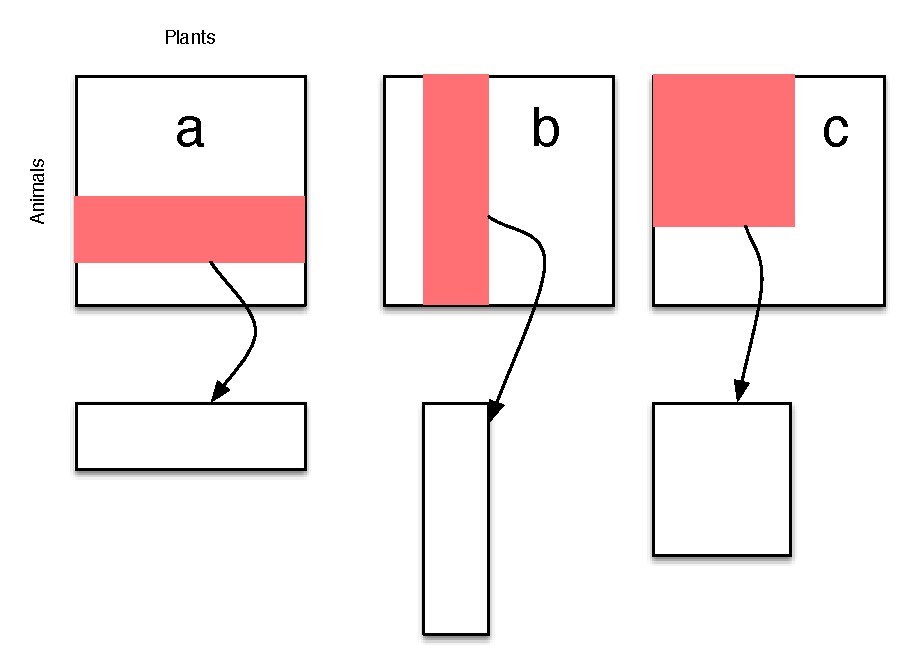
\includegraphics[keepaspectratio,width=\textwidth,height=0.75\textheight]{../figures/Fig2.pdf}
\caption{Figure 2. Sampling species interactions in natural communities. Suppose an assemblage with $A= 3$ animal species (red, species 1--3 with three, two, and 1 individuals, respectively) and $P= 3$ plant species (green, species a-c with three individuals each) (colored balls), sampled with increasing effort in steps 1 to 6 (panels). In Step 1 we record animal species 1 and plant species 1 and 2 with a total of three interactions (black lines) represented as two distinct interactions: $1-a$ and $1-b$. As we advance our sampling (panels 1 to 6, illustrating e.g., additional sampling days) we record new distinct interactions. Note that we actually sample and record interactions among individuals, yet we pool the data across species to get a species by species interaction matrix.}
\end{figure}

Our sampling above would have resulted in a vector $n= [n_1 ... n_C]'$ where $n_i$ is the number of records in the $i^{th}$ class. As stressed by Bunge \& Fitzpatrick \citep{Bunge:1993ux}, however, the $i^{th}$ class would appear in the sample if and only if $n_i > 0$, and we don't know \emph{a priori} which $n_i$ are zero. So, $n$ is not observable. Rather, what we get is a vector $c= [c_1 ... c_n]'$ where $c_j$ is the number of classes represented $j$ times in our sampling: $c_1$ is the number of singletons, $c_2$ is the number of twin pairs, $c_3$ the number of triplets, etc. The problem thus turns to be estimating the number of distinct classes $C$ from the vector of $c_j$ values.
 Estimating the number of interactions with resulting robust estimates of network parameters is a central issue in the study of ecological interaction networks \citep{E31/2562}\citep{Bascompte:2014to}.

\chapter{Asymptotic diversity estimates}
\label{asymptoticdiversityestimates}

Let's assume a sampling of the diversity in a specific locality, over relatively homogeneous landscape where we aim at determining the number of species present for a particular group of organisms. To do that we carry out transects or plot samplings across the landscape, adequately replicated so we obtain a number of samples. Briefly, $S_{obs}$ is the total number of species observed in a sample, or in a set of samples. $S_{est}$ is the estimated number of species in the community represented by the sample, or by the set of samples, where $est$ indicates an estimator. With abundance data, let $S_k$ be the number of species each represented by exactly $k$ individuals in a single sample. Thus, $S_0$ is the number of undetected species (species present in the community but not included in the sample), $S_1$ is the number of singleton species, $S_2$ is the number of doubleton species, etc. The total number of individuals in the sample would be:\\
$$n = 􏰢\sum_{k=1}^{S_{obs}}S_k$$\\
A frequently used asymptotic, bias corrected, estimator is $S_{Chao}$ \citep{Hortal:2006dc}\citep{Chao:2005wp}\citep{Colwell:2009}: 

$$S_{Chao}= S_{obs} + \frac{S_1 (S_1 −1)}{2(S_2 +1)}$$ 

Another frequently used alternative is the Chao2 estimator, $S_{Chao2}$ \citep{Gotelli:2001uo}, which has been reported to have a limited bias for small sample sizes \citep{Colwell:1994vt}\citep{Chao:2005wp}: 

$$S_{Chao2}= S_{obs} + \frac{S_1^2}{2S_2}$$ 

A plot of the cumulative number of species recorded, $S_n$, as a function of some measure of sampling effort (say, $n$ samples taken) yields the species accumulation curve (SAC) or collector's curve \citep{Colwell:1994vt}. Such a curve eventually reaches an asymptote converging with $S_{est}$. In an analogous way, interaction accumulation curves (IAC), analogous to SACs, can be used to assess the robustness of interactions sampling for plant-animal community datasets \citep{E31/2562}\citep{Jordano:2009c}\citep{Olesen:2011a}. 

\chapter{Assessing sampling effort when recording interactions}
\label{assessingsamplingeffortwhenrecordinginteractions}

The basic method we can propose to estimate sampling effort and explicitly show the analogues with rarefaction analysis in biodiversity research is to vectorize the interaction matrix $AP$ so that we get a vector of all the possible pairwise interactions that can occur in a community of $A$ animal species and $P$ plant species.
 The new ``species'' we aim to sample are the interactions. So, if we have in our community \emph{Turdus merula} ($Tm$) and \emph{Rosa canina} ($Rc$) and \emph{Prunus mahaleb} ($Pm$), our problem will be to sample 2 new ``species'': $Tm-Rc$ and $Tm-Pm$. In general, if we have $A= 1... i$ , animal species and $P = 1... j$ plant species, we'll have a vector of ``new'' species to sample: $A_1P_1, A_1P_2,... A_2P_1, A_2P_2, ... A_iP_j$. We can represent the successive samples where we can potentially get records of these interactions in a matrix with the vectorized interaction matrix and columns representing the successive samples we take (Table 1). This is simply a vectorized version of the interaction matrix.

\begin{table}[htbp]
\centering
\small
\caption{Table 1. A vectorized interaction matrix.}
\label{table1.avectorizedinteractionmatrix.}
Interaction&Sample1&Sample2&Sample3\\
\midrule
A1 - P2&12&2&0\\
A1 - P2&0&0&0\\
{\ldots}&{\ldots}&{\ldots}&{\ldots}\\
A5 - P3&5&0&1\\
A5 - P4&1&0&1\\
{\ldots}&{\ldots}&{\ldots}&{\ldots}\\
A\textsubscript{i} - P\textsubscript{i}&1&0&1\\

\bottomrule

\end{table}

Rarefaction analysis comes up immediately with this type of dataset. In addition, we should discuss the problem of rarifying the interaction matrix itself. I mean, are we able to estimate how robust has been the sampling of a given interaction matrix. This would be useful to assess the robustness of information already available, even with no data on sampling effort or with no access to the original individual samples.

\begin{verbatim}
We can discuss whether rarefaction estimates for interactions would be better obtained from sample-based simulations or individual based simulations. Sample-based simulations would require access to original raw data.
\end{verbatim}

\chapter{Discussion}
\label{discussion}

\section{Concluding Remarks}
\label{concludingremarks}

\chapter{\textbf{Acknowledgements}.}
\label{acknowledgements.}

I am indebted to Alfredo Valido, Jordi Bascompte, Thomas Lewinshon, John N. Thompson, Nick Gotelli, Carsten Dormann, and Paulo R. Guimarães Jr. for useful and thoughtful comments and discussion at different stages of this manuscript. The study was supported by a Junta de Andalucía Excellence Grant (RNM--5731), as well as a Severo Ochoa Excellence Award from the Ministerio de Economía y Competitividad (SEV--2012--0262). The Agencia de Medio Ambiente, Junta de Andalucía, provided generous facilities that made possible my long-term field work in different natural parks.

\begin{center}\rule{3in}{0.4pt}\end{center}


\chapter{Tables}
\label{tables}

\section{Table 1. A vectorized interaction matrix.}
\label{table1.avectorizedinteractionmatrix.}

\section{Table 2. \emph{*}.}
\label{table2..}

\chapter{Figures}
\label{figures}

\section{\textbf{Figure 1}. Sampling ecological interaction networks usually focus on different types of subsampling the full network. a) all the potential plants interacting with a subset of the animals (e.g., studying just the hummingbird-pollinated flower species in a community; b) all the potential animal species interacting with a subset of the plant species (e.g., studying the frugivore species feeding on figs \emph{Ficus} in a community); and c) sampling a subset of all the potential animal species interacting with a subset of all the plant species (e.g., studying the plant-frugivore interactions in the rainforest understory).}
\label{figure1.samplingecologicalinteractionnetworksusuallyfocusondifferenttypesofsubsamplingthefullnetwork.aallthepotentialplantsinteractingwithasubsetoftheanimalse.g.studyingjustthehummingbird-pollinatedflowerspeciesinacommunityballthepotentialanimalspeciesinteractingwithasubsetoftheplantspeciese.g.studyingthefrugivorespeciesfeedingonfigsficusinacommunityandcsamplingasubsetofallthepotentialanimalspeciesinteractingwithasubsetofalltheplantspeciese.g.studyingtheplant-frugivoreinteractionsintherainforestunderstory.}

\section{\textbf{Figure 2}. Sampling species interactions in natural communities. Suppose an assemblage with $A= 3$ animal species (red, species 1--3 with three, two, and 1 individuals, respectively) and $P= 3$ plant species (green, species a-c with three individuals each) (colored balls), sampled with increasing effort in steps 1 to 6 (panels). In Step 1 we record animal species 1 and plant species 1 and 2 with a total of three interactions (black lines) represented as two distinct interactions: $1-a$ and $1-b$. As we advance our sampling (panels 1 to 6, illustrating e.g., additional sampling days) we record new distinct interactions. Note that we actually sample and record interactions among individuals, yet we pool the data across species to get a species by species interaction matrix.}
\label{figure2.samplingspeciesinteractionsinnaturalcommunities.supposeanassemblagewitha3animalspeciesredspecies1-3withthreetwoand1individualsrespectivelyandp3plantspeciesgreenspeciesa-cwiththreeindividualseachcoloredballssampledwithincreasingeffortinsteps1to6panels.instep1werecordanimalspecies1andplantspecies1and2withatotalofthreeinteractionsblacklinesrepresentedastwodistinctinteractions:1-aand1-b.asweadvanceoursamplingpanels1to6illustratinge.g.additionalsamplingdayswerecordnewdistinctinteractions.notethatweactuallysampleandrecordinteractionsamongindividualsyetwepoolthedataacrossspeciestogetaspeciesbyspeciesinteractionmatrix.}

\section{\textbf{Figure 3}.}
\label{figure3.}

\begin{center}\rule{3in}{0.4pt}\end{center}


\chapter{Online Support Material}
\label{onlinesupportmaterial}

\begin{center}\rule{3in}{0.4pt}\end{center}


\chapter{Methods}
\label{methods}

\begin{center}\rule{3in}{0.4pt}\end{center}


\chapter{References for Online Material}
\label{referencesforonlinematerial}

\begin{center}\rule{3in}{0.4pt}\end{center}


\chapter{NOTES}
\label{notes}

\section{REFS}
\label{refs}

\subsection{Chacoff et al.}
\label{chacoffetal.}

One of the major current challenges is to understand sampling accuracy and how to improve it.
Detection increased with increasing sampling effort and flower abundance, but decreased with increasing selectiveness, length of the flowering period and degree (Table 3). In addition, interactions meant that for plant species with low degree (i.e. specialists), detection decreases with increasing flowering length while it increases for plants with high degree (i.e. generalists) (Fig. 4a). Similarly, for plant species with high selectiveness, detection increases with increasing length of flowering period, while it decreases with decreasing selectiveness (Fig. 4b); finally, for plants with low degree, detection decreases with increasing flower abundance while it increases with increasing degree (Fig. 4c). Thus, plant species with either low degree, high selectivity and long flowering period or generalists species with low flower abundance and short flowering span had the lowest detection of the estimated number of interactions.
We still need to disentangle true ecological factors, such as species abundance and dynamics, from sampling biases (Vázquez et al. 2009a) to improve our ability to detect interactions in mutualistic networks.

\subsection{Section 2 - Text from PUP book.}
\label{section2-textfrompupbook.}

\subsection{Sampling and robustness of network parameters}
\label{samplingandrobustnessofnetworkparameters}

\% PJ: 2May2010

For instance, a random accumulator function (library vegan in the R Package; \textbackslash{}citep\{R10\}) which finds the mean IAC and its standard deviation from random permutations of the data, or subsampling without replacement \textbackslash{}citep\{GotCol01\} can be used to estimate the expected number of pairwise interactions included in a given sampling of records (Fig. 1C). We start with a vectorized interaction matrix \textbackslash{}citep\{Jor09\} representing the pairwise interactions (rows) recorded during a cumulative number of censuses or sampling periods (columns), in a way analogous to a biodiversity sampling matrix with species as rows and sampling units (e.g., quadrats) as columns. This procedure plots the accumulation curve for the expected number of pairwise interactions recorded with increasing sampling effort (Fig. 1C).

Not all potential links among species in ecological networks can be recorded during sampling. Often, adjacency matrices are used to characterize complex networks, and these matrices are frequently sparse, i.e., they are densely populated with zeroes. Unobserved interactions are represented by zeroes and belong to two categories. Missing interactions actually exist but may require additional sampling or a variety of methods to be observed. Forbidden links, on the other hand, arise due to biological constraints limiting interactions and remain unobservable in nature, irrespectively of sampling effort \textbackslash{}citep\{JBO03,Olesen:2010a\}. Forbidden links are non-occurrences of pairwise interactions that can be accounted for by biological constraints, such as spatio-temporal uncoupling, size or reward mismatching, foraging constraints (e.g., accessibility), and physiological-biochemical constraints \textbackslash{}citep\{Jordano:1987,Olesen:2010a\}. Temporal uncoupling, for example, takes place when phenophases of potentially interacting species do not overlap \textbackslash{}citealt[e.g.,][]\{Fabina:2010\} (Fig. 1A, B). Thus forbidden links can be defined as structural zeroes in the adjacency matrix describing a complex network. Therefore, the potential links that can actually be observed in an interaction matrix of \textbackslash{}textit\{A\} and \textbackslash{}textit\{P\} animal and plant species is well below the total size of the matrix, \textbackslash{}textit\{AP\}. Two elements of inference are required in the analysis of missing interactions in plant-animal interaction networks: first, a critical analysis of sampling robustness; second, detailed natural history information on the participant species that allows the inference of biological constraints.

It is noteworthy that null models of interaction matrices, either binary or weighted, do not account for the presence of forbidden links in empirical networks. For instance, the computation of connectance refers the observed number of interactions $I$ to the total \textbackslash{}textit\{possible\} or \textbackslash{}textit\{potential\} interaction in a matrix with $A$ animal species and $P$ plant species: $AP$. Yet, given the presence of forbidden links in empirical networks, $AP$ obviously overestimates the \textbackslash{}textit\{potential\} number of interactions, simply because the actual \textbackslash{}textit\{possible\} number is well below the maximum indicated by the product $AP$. It is no surprise that null models based on randomizations of the interaction matrix often yield a low frequency of expected zeroes \textbackslash{}citep\{Bluthgen:2008p7146\}, the simulation algorithm just fills in cells that never should get a non-zero expected value. As a result, a typical result of these simulated matrices is a larger connectance of the null matrices relative to the empirical ones \textbackslash{}citep\{Bluthgen:2008p7146\}. Future work on null algorithms for interaction matrices should take into account these effects of forbidden links. A potential avenue would be to estimate the actual frequency of forbbiden interactions in real-world assemblages \textbackslash{}citep\{Olesen:2010a\} and correct the filling of the null matrices by this frequency.

A side-effect of forbidden links is what we call ``edge-interactions''. If forbidden interactions, like those among species with non-overlapping phenophases (Fig. 1A) are non-observable by definition, what about those interactions among species that just marginally overlap their phenophases (Fig. 1A, B)? Imagine a flower species at the end of the flowering period, when very few individuals in the population have very few flowers still open. Then consider a newly emerging insect pollinator whose phenophase occurs slightly later than these flowers (e.g., the interaction between sp. $a_3$ and $p_3$ in Fig. 1A). 

Links between super-rare species in a network can be extremely difficult to detect, largely because of an intrinsically low species-encounter rate in the field. According to our link classification \textbackslash{}citep\{Olesen:2010a\}, these interactions are missing, i.e. not accounted for by any implied biological constraint. However, very low abundance may also limit actual interactions to occur if the probability of interspecific interaction is constrained by the intrinsically low probability of interspecific encounter \textbackslash{}citep\{Mac72\}. The extent of phenological coupling or overlap is a temporal equivalent to encounter rate. If two species overlap phenologically by one-few days (e.g., species $a_3$ and $p_3$ in Fig. 1B) an interaction is possible, but extremely unlikely. This is even further enforced by an intrinsically low abundance of the interacting species at the onset and end of their phenophases. Thus, besides the unobservable links accounted for by forbidden interactions, many links could remain missing simply because of an intrinsically low probability of interspecific encounter. This underscores the crucial point of assessing how robust is the sampling of interactions. The relevant point here in relation to sampling is that, contrary to recent interpretations \textbackslash{}citep\{Dorado:2011\}, many zeroes in interaction matrices should not be considered artifacts of undersampling or passive sampling affected by abundance variations of the component species \textbackslash{}citep\{BMB06\}. This is especially evident in robustly sampled datasets, where a high fraction of structural zeroes are expected despite intensive sampling.

Sampling effort also influences the robustness of parameter estimation in network analyses. As noted earlier in this chapter, there is a high turnover in the number of species and interactions through years. Therefore, how robust are the indices of network structure is a relevant question given the noise and sampling errors. The first paper tackling this question in relation to nestedness was \textbackslash{}citet\{NieBas07\}. These authors designed an experimental approach to a pollination site near Siljan in South-East Norway. Sampling effort was controlled both in time and space. Twelve study sites of 20 $\times$ 20 meters were evenly distributed among forest stands of different maturity. First, results were quite equivalent for spatial and temporal sampling. While the number of species and interactions kept growing, absolute nestedness seems to be much more stable. Since absolute nestedness depends on number of species and interactions, \textbackslash{}cite\{NieBas07\} also calculated relative nestedness (the value of nestedness for a given matrix compared with the average value for a population of randomizations of such a matrix). Relative nestedness increases with sampling effort but reaches an asymptotic level well within the extent of the sampling effort considered. That is, nestedness would remain quite constant and no changes would be observed if one was sampling more days or plots beyond the asymptotic value. Of course the exact level of spatial and temporal sampling that is enough to characterize nestedness will depend on the study system, but the point is that nestedness is much more convergent than connectance or number of species and interactions. 

Missing links are a characteristic feature of all plant-animal interaction networks. Important natural history details explain a fraction of them, resulting in unobservable interactions (i.e., forbidden interactions) that define structural zeroes in the interaction matrices. Focusing on sampling interactions is a way to monitor biodiversity beyond the simple enumeration of component species and to develop efficient and robust inventories of functional interactions. Focussing just on the realized interactions or treating missing interactions as the expected unique result of sampling bias would miss important components to understand how mutualisms coevolve within complex webs of interdependence among species. 

\begin{center}\rule{3in}{0.4pt}\end{center}


\chapter{REFERENCES}
\label{references}

\section{REFRENCES TO ADD}
\label{refrencestoadd}

\newpage
%%%%%%%%%%%%%%%%%%%%%%%%%%%%%%%%%%%%%%%%%%%%%%%%%%%%%%%%%%%%%%%%%% References
%%% Unnumbered Literature Cited
\bibliographystyle{ecology} % Choose AREES style for bibliography
\bibliography{refs}
%%%%%%%%%%%%%%%%%%%%%%%%%%%%%%%%%%%%%%%%%%%%%%%%%%%%%%%%%%%%%%%%%%%%%%%%%%%%%
%
\end{linenumbers}
\end{document}